\documentclass[tikz,border=3mm,multi=tikzpicture]{standalone}
\usepackage[utf8]{inputenc}
\usepackage[T1]{fontenc}
\usepackage{helvet}
\renewcommand{\familydefault}{\sfdefault}
\usepackage{tikz}
\usetikzlibrary{arrows.meta,positioning}
\begin{document}

\tikzset{every node/.append style={font=\sffamily\small}}

% TikZ 1
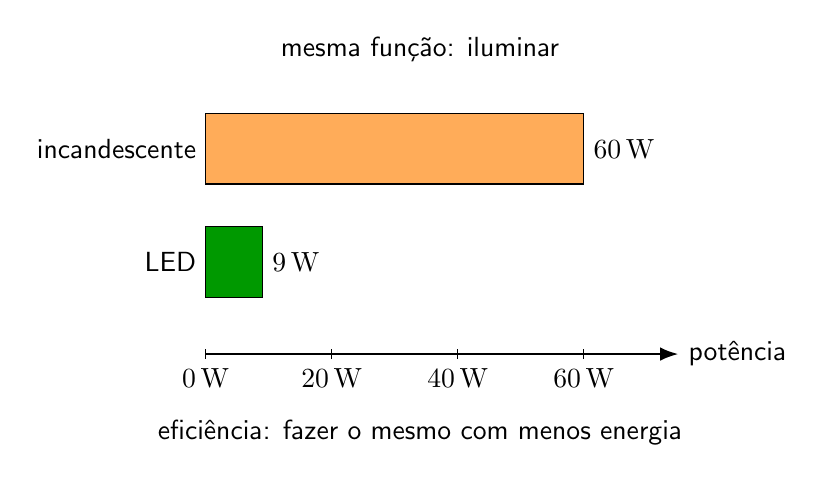
\begin{tikzpicture}[x=0.08cm,y=0.18cm,>=Latex]
  \draw[->,thick] (0,0) -- (75,0) node[right] {potência};
  \foreach \x in {0,20,40,60}{
    \draw (\x,0.35) -- (\x,-0.35);
    \node[below] at (\x,-0.35) {$\x\,\mathrm{W}$};
  }
  \draw[fill=orange!65] (0,12) rectangle (60,17);
  \node[left] at (0,14.5) {incandescente};
  \node[right] at (60,14.5) {$60\,\mathrm{W}$};
  \draw[fill=green!60!black] (0,4) rectangle (9,9);
  \node[left] at (0,6.5) {LED};
  \node[right] at (9,6.5) {$9\,\mathrm{W}$};
  \node[align=center,above] at (34,20) {mesma função: iluminar};
  \node[align=center,below] at (34,-4) {eficiência: fazer o mesmo com menos energia};
\end{tikzpicture}

% TikZ 2
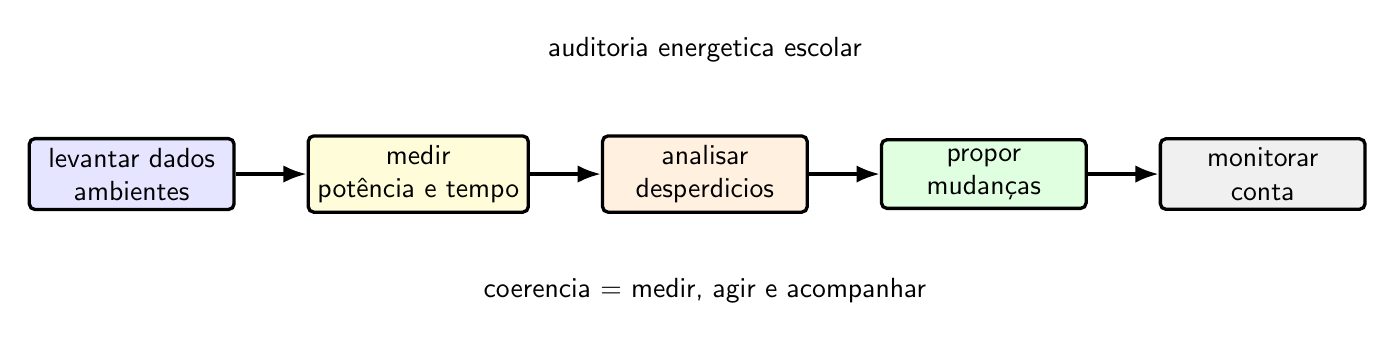
\begin{tikzpicture}[>=Latex,node distance=0.75cm]
  \tikzstyle{box}=[draw,rounded corners=2pt,minimum width=2.6cm,minimum height=0.85cm,align=center,very thick]
  \node[box,fill=blue!10] (lev) {levantar dados\\ambientes};
  \node[box,fill=yellow!15,right=0.9cm of lev] (med) {medir\\potência e tempo};
  \node[box,fill=orange!12,right=0.9cm of med] (anal) {analisar\\desperdicios};
  \node[box,fill=green!12,right=0.9cm of anal] (prop) {propor\\mudanças};
  \node[box,fill=gray!12,right=0.9cm of prop] (mon) {monitorar\\conta};
  \draw[very thick,->] (lev) -- (med);
  \draw[very thick,->] (med) -- (anal);
  \draw[very thick,->] (anal) -- (prop);
  \draw[very thick,->] (prop) -- (mon);
  \node[align=center,above=0.8cm of anal] {auditoria energetica escolar};
  \node[align=center,below=0.7cm of anal] {coerencia = medir, agir e acompanhar};
\end{tikzpicture}

\end{document}
